\chapter{Architectural design}
% overview of the project
% high level view of the project - Present a bird’s-eye view of the project architecture, highlighting key components and their interactions, add diagrams for clarity
% view of the project in the context of the ecommerce company - how the architecture aligns with the business goals and operational needs of the e-commerce company. Include considerations like scalability, maintainability, and security.
% view of the project in the context of the ecommerce customer -  how the architectural design impacts the customer experience. Focus on usability, performance, and reliability from the customer’s perspective
% multitenancy - definitive design considerations and implementation strategy for supporting multitenancy in the architecture. 
% serverless - role and benefits of serverless architecture in the project. Discuss how serverless components are utilized for scalability, cost-effectiveness, and operational efficiency.

The architecture of robust software is not just the description of the technology used in the development process; it is the blueprint of the project.
As we transition from the foundational requirements outlined in the previous chapter \ref{sec:requirements}, we can start designing the overall project.
This chapter aims to present a high-level architecture of how communication is orchestrated between all services and key components of the project.
As stated in \cite{sommervilleSW}, the establishment of a robust architecture in the early stages of development is the key.
Because while refactoring components due to minor changes of requirements in the life-cycle of the software is usually relatively easy, refactoring a system architecture is likely to be quite expensive.
The reader can intuitively find parallel between house architecture and software architecture. 
Injection of foundations, or making foundations more robust while house sits on them will always be much more expensive and certainly with more compromises than when building a new house with a proper foundations.

%Since we are building an application whose purpose is to live in the cloud, serve multiple tenants, send emails, and provide a front-end with graphical user interface, we can roughly estimate what the architecture will look like.
%We will definitely need an application providing the user interface, functionalities, or the business logic, and store somewhere user data.

Since we are developing a web application designed for cloud deployment, several key architectural components become essential to meet our goals.
The aim is to create a solution that not only serves multiple tenants within a single instance, but also manages to send emails reliably and provides an intuitive graphical interface.
Given these constraints, we can foresee the foundational structure of our architecture.

As the core, our architecture will comprise three principal components:
\begin{enumerate}
    \item \textbf{User Interface:} A user-friendly front-end that serves as the primary interaction point for users and customers (see definition of actors in section \ref{sec:requirements-actors}). This component is essential for information presentation and user input.
    \item \textbf{Business Logic Layer:} The backbone of our platform, where the essential functionalities and operational logic reside. This layer will encapsulate all the rules needed to run the core processes of our service. From handling user requests to processing data and orchestrating email notifications.
    \item \textbf{Data Storage:} A database system designed to store, manage, and retrieve user data, as well as application-specific information. Given the multi-tenant nature of the platform, the database architecture will be designed to ensure data isolation, integrity, and security for each tenant.
\end{enumerate}

To visualise the high-level approach of the few components mentioned above, we will use a diagram of layered architecture. 
It is an architectural approach to organise the system into layers with different orders. 
In our case, the layered architecture would look as visualised in Figure \ref{img03:layered_architecture_diagram}.

\begin{figure}[H]\centering
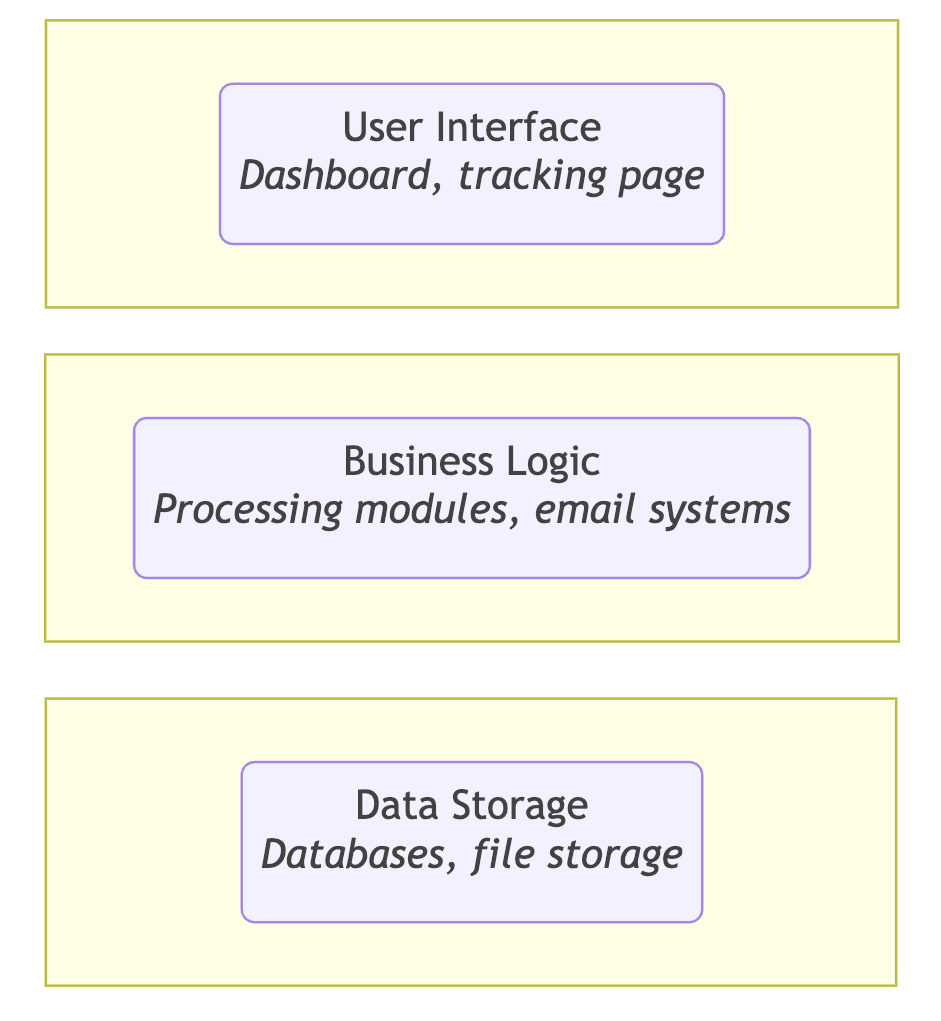
\includegraphics[width=80mm]{img/chap03/fig_layered_architecture_mermaid.png}
\caption{High-level layered architecture diagram}
\label{img03:layered_architecture_diagram}
\end{figure}

%graph TD;
%    UI[User Interface] --> BL[Business Logic];
%    BL --> DS[Data Storage];

%    subgraph UI_Layer[ ]
%        UI(User Interface<br><i>Dashboard, tracking page</i>)
%    end

%    subgraph BL_Layer[ ]
%        BL(Business Logic<br><i>Processing modules, email systems</i>)
%    end

%    subgraph DS_Layer[ ]
%        DS(Data Storage<br><i>Databases, file storage</i>)
%    end

%    style UI_Layer fill:#f9f,stroke:#333,stroke-width:2px
%    style BL_Layer fill:#ccf,stroke:#333,stroke-width:2px
%    style DS_Layer fill:#cfc,stroke:#333,stroke-width:2px

\section{Architectural Decisions}
\label{sec:architectural-decisions}
% Describe decisions made to desing the applicaiton
Before diving into the specifics of the application architecture, it is important to understand the foundational decisions that shape the overall architectural and implementation design of the platform.
These decisions are mainly influenced by non-functional requirements found in section \ref{subsec:nonfunctional-requirements}, current trends, and author's subjective experience.

\subsection{Accommodating Serverless Architecture}
A key decision in the project's backend architectural design is the adoption of a serverless architecture.
This approach allows to focus on application development without the overhead of managing infrastructure, allowing improved scalability and cost efficiency.


\subsection{API-first Approach}
Prioritizing an API to be a robust backbone of the platform.
Allowing to serve a wide range of frontend interfaces and preferably a third-party integrations via well-documented Public API.


\subsection{Choosing a Multi-Tenant Data Model}
One of the key requirements is to serve multiple users from a single instance of the application due to the optimisation of operational costs, complexity, and maintainability.
This decision influences the database schema and application logic, ensuring data isolation.
The chosen approach was a single database, a single schema approach, which required data isolation at the query level. More information on approaches for multi-tenancy is described in Section \ref{sec:different-approaches-for-multitanency}.
The main unit within the chosen approach is the Project entity represented within the data model in the \ref{subsubsec:data-model} section.
This entity allows data to be shared between multiple users added by the owner of a given project.
This ensures data security, as all filtering at and above the database level is done based on the project the user has access to.


\subsection{Ensuring Extensibility and Integration Capability}
Recognizing the dynamic nature of the e-Commerce industry, architecture is designed with extensibility and integration capability at its core. 
The system needs to accommodate new shipping carriers and integrate with external \ac{ERP} systems.


\section{Application Architecture}
\label{sec:application-architecture}
% overview of the architecture of Parcelsync
This section dives into various aspects of the platform's architecture, laying out a design prioritizing maintainability and scalability. For a high-level diagram of the system, see Figure \ref{img03:c4_container_diagram_software_sytem}.
The architecture is intended to accommodate cloud-based, multi-tenant environment.

\begin{figure}[H]\centering
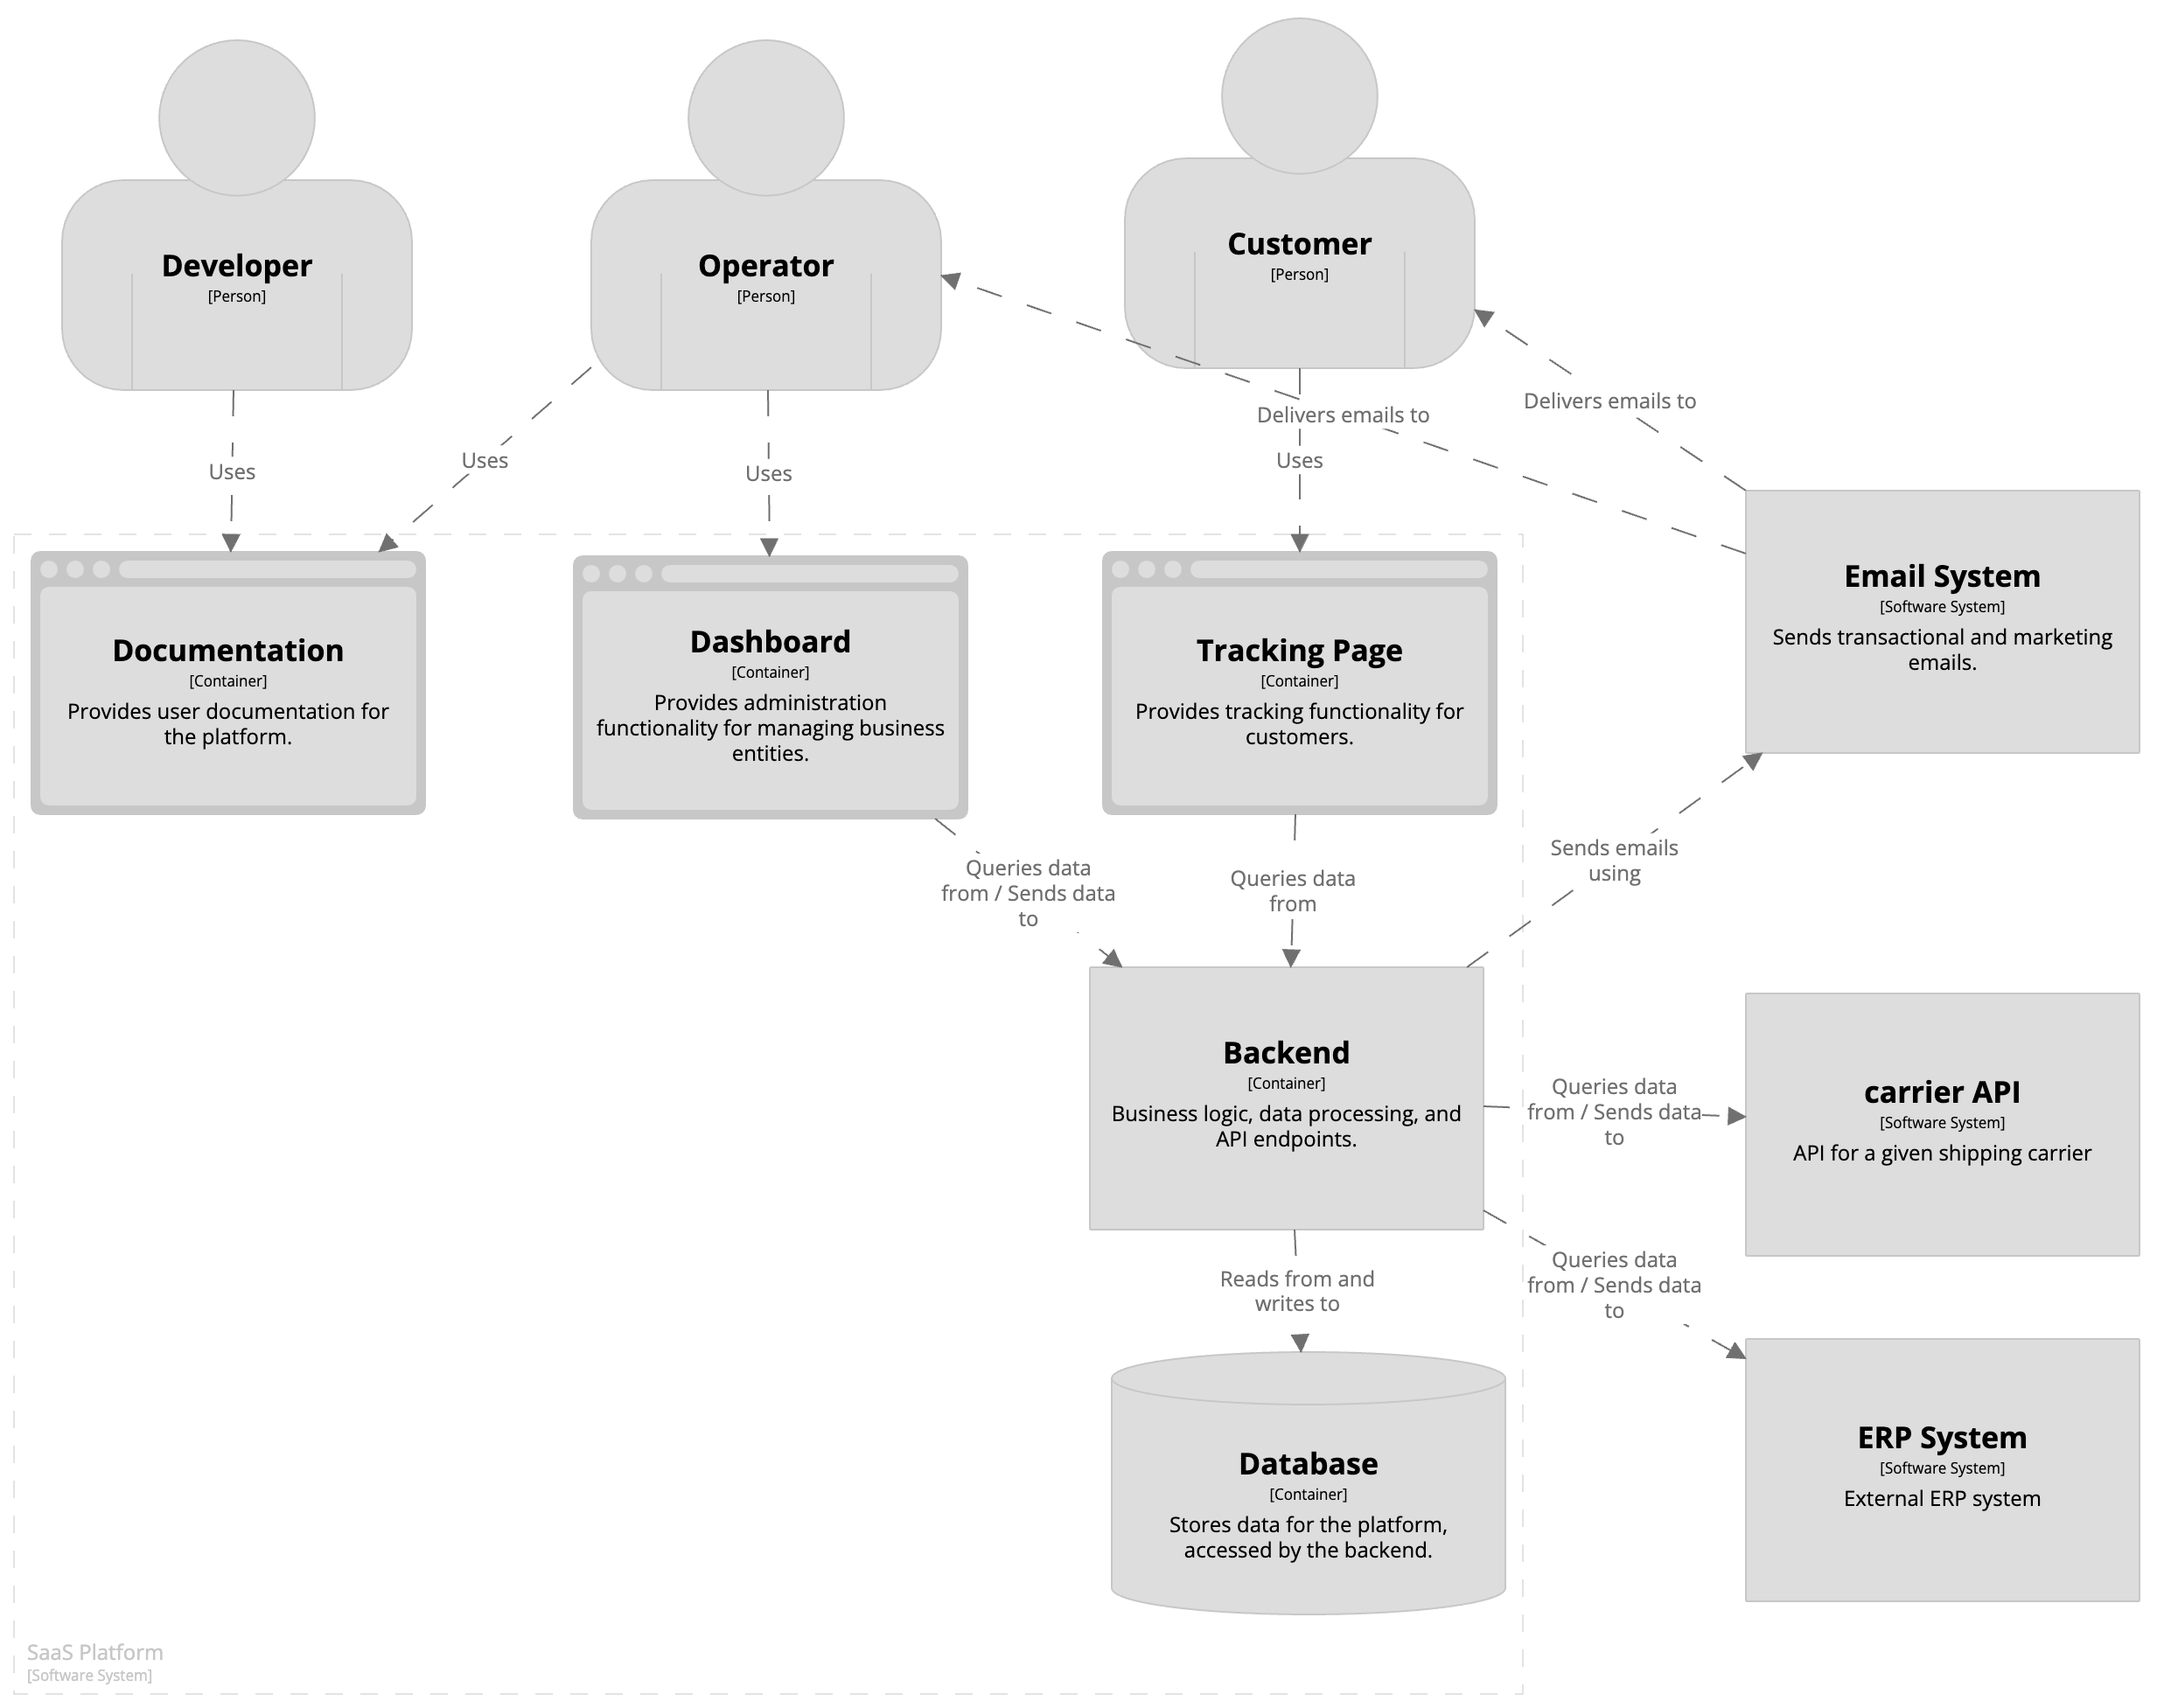
\includegraphics[width=140mm]{img/chap03/fig_architecture.png}
\caption{C4 container diagram of the software system}
\label{img03:c4_container_diagram_software_sytem}
\end{figure}

\subsection{Backend}
\label{subsec:backend}
% backend design descripiton - backend architecture in detail, including technologies used, server configurations, API design, and integration strategies
At the heart of the platform is a backend component designed to provide business logic, data processing and external communication.
The backend is structured to efficiently provide and share functionality within the component or through a set of REST API methods intended either for an internal integration of frontend components or external integrations to third-party systems.
Without diving into implementation details, the backend is designed in a way that allows it to run in a serverless environment.
The backend serves as the exclusive component directly connected to the database, making it the singular source for all \ac{CRUD} operations.
This design decision not only simplifies data management but also reinforces the security and integrity of the database.

\subsubsection{External carrier integrations}
An essential feature of backend is its capability to integrate with different shipping carriers.
This feature enables data transfer between carrier and platform, as well as label and waybill generation.
\begin{itemize}
    \item \textbf{Modular integration design:} Carrier integrations are implemented as modular components within the backend without impacting the core system.
    \item \textbf{Unified interface:} Despite the diversity of carrier APIs, the backend should abstract these differences, presenting a unified interface to the rest of the platform. This significantly simplifies the process of adding new carriers and maintaining existing ones.
    \item \textbf{Data unification:} The backend is responsible for unification of data across different carriers, translating tracking statuses into a standardised format used throughout the platform.
\end{itemize}

\subsubsection{Scheduled tasks}
To support operations that require periodic execution, such as synchronising shipment statuses or triggering the sending of email status, the backend includes a mechanism for creating scheduled tasks in a serverless environment.

\subsubsection{Public API}
A key feature of the backend is its publicly exposed Public REST API that offers a gateway for third-party integrations.
The API is documented in the OpenAPI specification.
This API facilitates secure and efficient communication. 

\subsection{Frontend}
\label{subsec:frontend}
% frontend design descripiton - frontend architecture, focusing on the user interface design, frontend frameworks, and how it interacts with the backend.
\subsubsection{Dashboard}
\subsubsection{Tracking page}
\subsection{Database}
\label{subsec:database}
 % database architecture, including the database model
\subsubsection{Data Model}
\label{subsubsec:data-model}
% in-depth look at the data model used in the project, relationship diagrams, data, and explanations of how data modeling supports the application's functionality
